\subsection{Use-case diagram and Use-case scenario}
\newpage
\begin{figure}[H]
    \begin{center}
        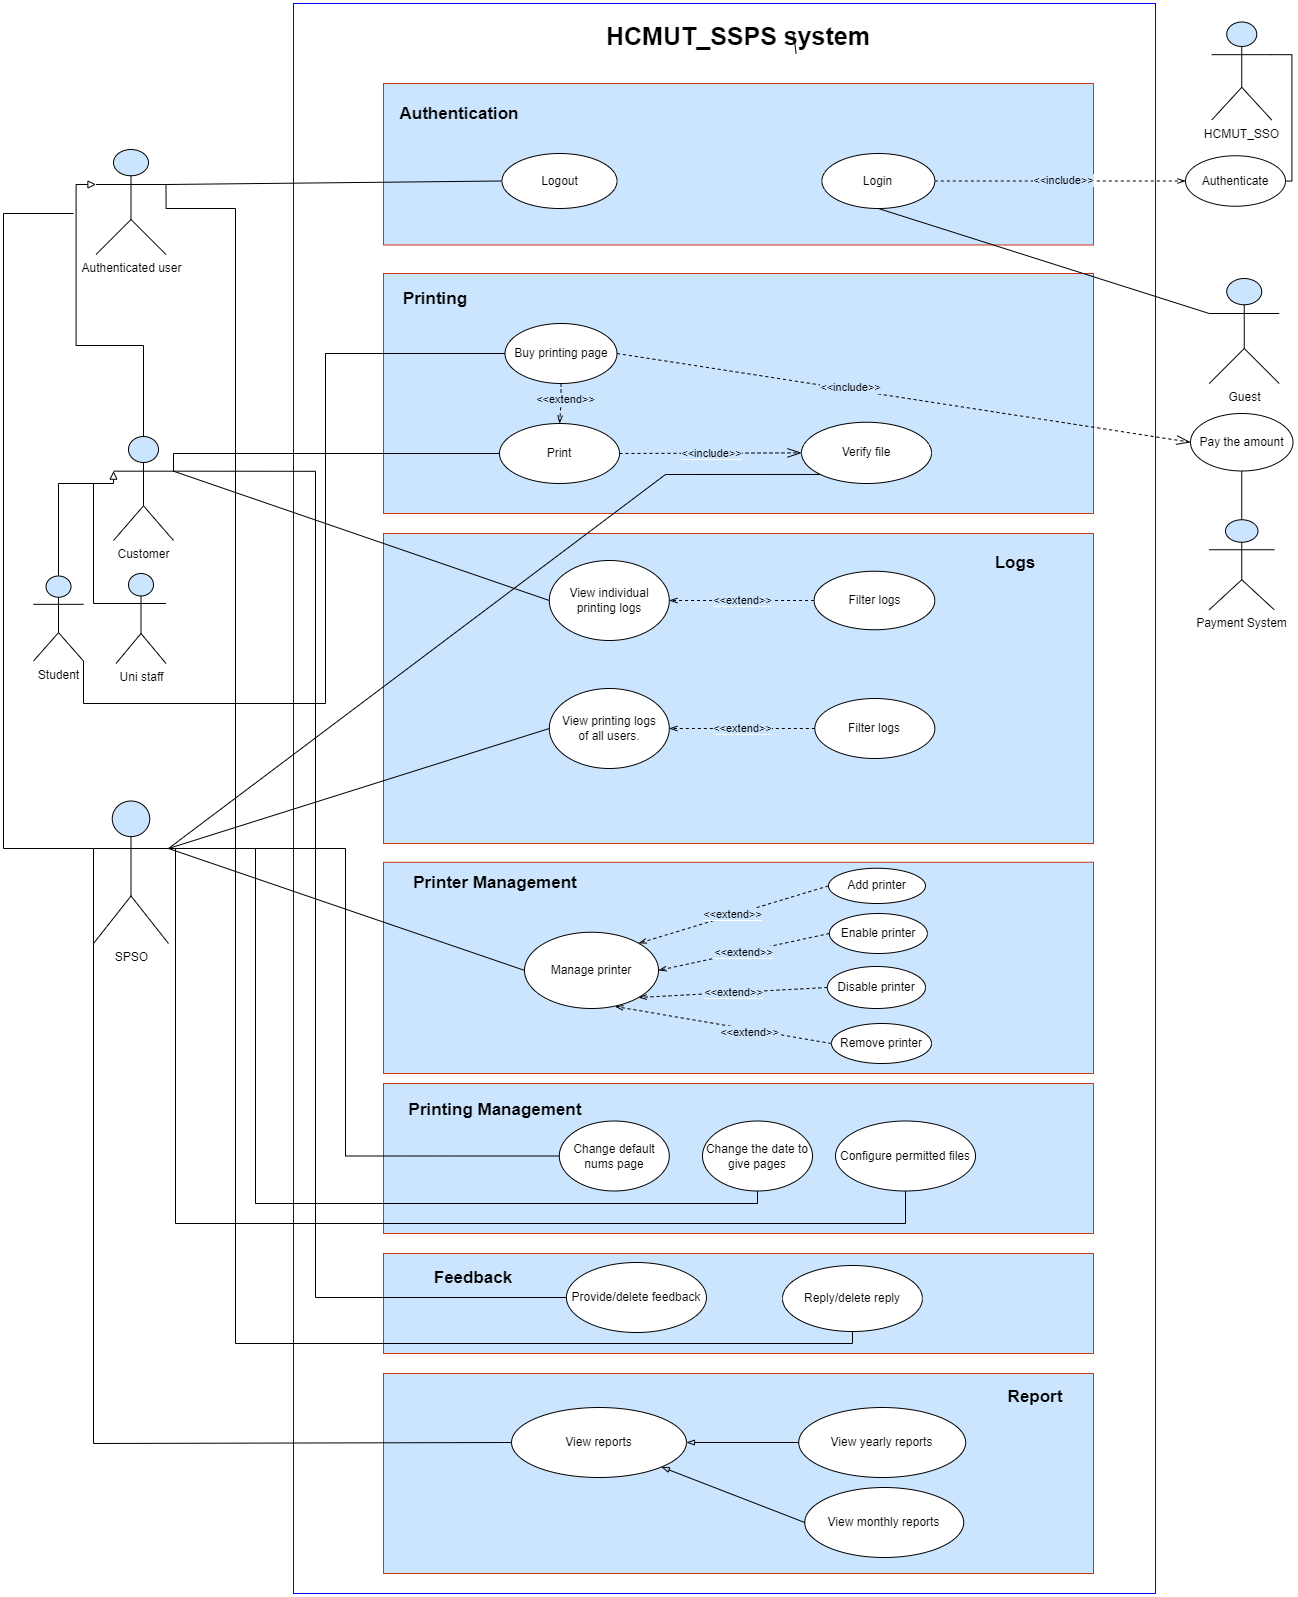
\includegraphics[width=0.9\textwidth]{Images/Requirement Elicitation/SPSS_system_Use-case.png}
        \caption{Use-case diagram cho hệ thống}
        \label{fig:arch}
    \end{center}
\end{figure}

\subsubsection{Xác thực}
\subsubsubsection{Use case diagram}
\begin{figure}[H]
    \begin{center}
        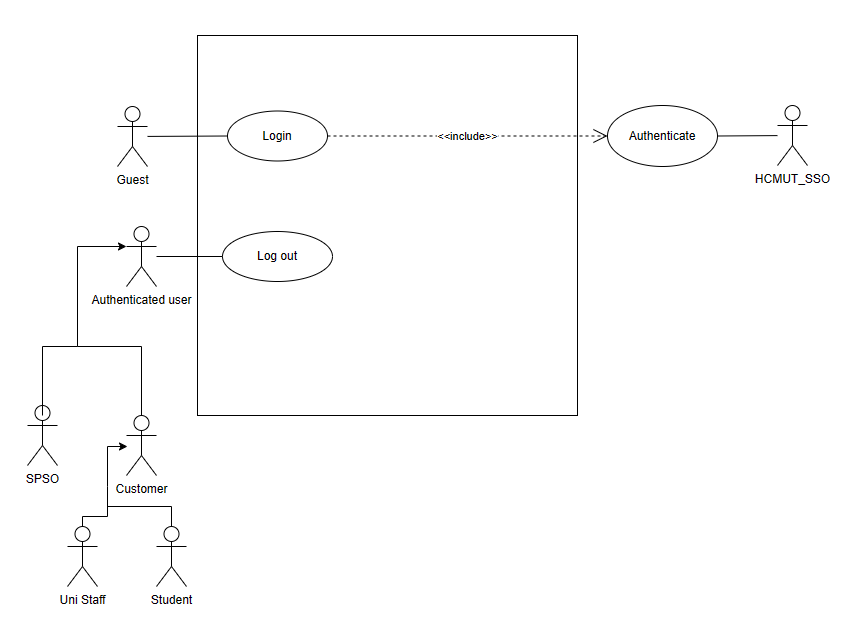
\includegraphics[width=1\textwidth]{Images/Requirement Elicitation/Authentication_Use-case.png}
        \caption{Use-case diagram cho chức năng xác thực tài khoản}
    \end{center}
\end{figure}
\pagebreak
\subsubsubsection{Use-case scenario}
\textbf{Use-case Login}\par
\vspace{0.5cm}
\begin{tabular}{|l|l|l|l|}
\hline Use case name: & \multicolumn{3}{|l|}{Login} \\
\hline Created by: & Nguyễn Đình Quang & Last updated by: &  Nguyễn Đình Quang \\
\hline Date created: & 28/09/2023 & Date last updated: & 30/09/2023\\
\hline Actors: & \multicolumn{3}{|l|}{ Authenticated User (SPSO và người dùng) } \\
\hline Description: & \multicolumn{3}{|l|}{$\begin{array}{l}\text{Use case này cho phép Guest đăng nhập vào hệ thống } \end{array}$} \\

\hline Trigger: & \multicolumn{3}{|l|}{$\begin{array}{l}\text{Click vào nút “Login” trên giao diện chính của website.} \end{array}$} \\
\hline Preconditions: & \multicolumn{3}{|l|}{$\begin{array}{l}\text {Guest chưa đăng nhập vào hệ thống} \\ \text{Guest dùng có tài khoản trên ứng dụng} \\ \text{Thiết bị của Guest có kết nối mạng} \end{array}$} \\
\hline Postconditions: & \multicolumn{3}{|l|}{$\begin{array}{l}\text {Guest đăng nhập thành công.} \end{array}$} \\
\hline Normal Flows: & \multicolumn{3}{|l|}{$\begin{array}{l}\text {1. Guest chọn "Login". } \\
\text {2. Hệ thống hiển thị giao diện đăng nhập. } \\
\text {3. Chọn đối tượng đăng nhập. } \\
\text {4. Guest nhập username và password. } \\
\text {5. Guest nhấn nút "Log in".  } \\
\text {6. Hệ thống xác thực thông tin đăng nhập. } \\
\text {7. Hệ thống cập nhật lại giao diện theo thông tin của tài khoản Guest. }\end{array}$} \\
\hline  Alternative Flows: & \multicolumn{3}{|l|}{} \\
\hline Exceptions: & \multicolumn{3}{|l|}{$\begin{array}{l}\textbf{E1: Tại bước 6 } \\
\text {6a: Guest nhập Username/ Password sai. } \\
\text {6b: Hệ thống hiển thị thông báo sai thông tin đăng nhập. } \\
\text {Quay lại bước 3 trong normal flows. } \end{array}$} \\
\hline Note and issues: & \multicolumn{3}{|l|}{$\begin{array}{l}
\text{Nếu User hiện đang đăng nhập, sau đó tiếp tục đăng nhập vào hệ thống } \\
\text{bằng thiết bị khác, thiết bị cũ sẽ không tự động bị đăng xuất} \end{array}$ } \\
\hline
\end{tabular}

\pagebreak
\subsubsection{In}
\subsubsubsection{Use-case diagram}
\begin{figure}[H]
    \begin{center}
        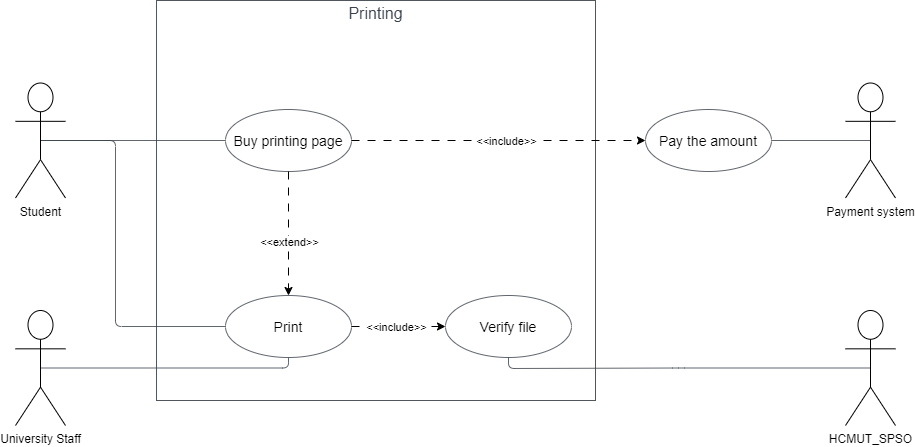
\includegraphics[width=1\textwidth]{Images/Requirement Elicitation/Printing_Use-case.png}
        \caption{Use-case diagram cho chức năng in tài liệu}
    \end{center}
\end{figure}

\subsubsubsection{Use-case scenario}
\pagebreak
\textbf{Use-case Print}\par
\vspace{0.5cm}
\begin{tabular}{|l|l|l|l|}
\hline Use case name: & \multicolumn{3}{|l|}{Print} \\
\hline Created by: & Trương Hoàng Nhật & Last updated by: &  Trương Hoàng Nhật \\
\hline Date created: & $27 / 09 / 2023$ & Date last updated: & $27 / 09 / 2023$\\
\hline Actors: & \multicolumn{3}{|l|}{ Student, University staff } \\
\hline Description: & \multicolumn{3}{|l|}{Cho phép người dùng upload và in tài liệu sau khi đã được kiểm duyệt} \\
\hline Trigger: & \multicolumn{3}{|l|}{ Người dùng nhấn vào nút "In ngay" ở thanh điều hướng } \\
\hline Preconditions: & \multicolumn{3}{|l|}{$\begin{array}{l}\text { - Người dùng đã có tài khoản trên hệ thống } \\
\text { - Người dùng tải lên tài liệu đã được kiểm duyệt } \\
\text { - Người dùng còn đủ số lượng giấy in trong tài khoản }\\
\text { -  Người dùng đã lựa chọn thời gian, vị trí máy in, cấu hình in. }\end{array}$} \\
\hline Postconditions: & \multicolumn{3}{|l|}{$\begin{array}{l}\text { Người dùng sẽ được xếp vào hàng chờ của máy in đã chọn } \end{array}$} \\
\hline Normal Flows: & \multicolumn{3}{|l|}{$\begin{array}{l}\text { 1. Người dùng chọn "In ngay" tại thanh điều hướng } \\
\text { 2. Hệ thống hiển thị giao diện để người dùng chọn máy in } \\
\text { 3. Người dùng lọc các thông tin của máy in (cơ sở, tòa, phòng) } \\
\text { 4. Hệ thống hiện danh sách các máy in khả dụng và số lượng người} \\
\text { \hspace{0.3cm} đang chờ trong hàng đợi của mỗi máy in} \\
\text { 5. Người dùng chọn vào máy cần in }\\
\text { 6. Người dùng upload file cần in lên hệ thống }\\
\text { 7. Hệ thống tiến hành kiểm duyệt file vừa được up } \\
\text { 8. Người dùng chọn thời gian in, định dạng cách thức in} \\
\text { 9. Người dùng xác nhận thao tác in} \end{array}$} \\
\hline  Alternative Flows: & \multicolumn{3}{|l|}{$\begin{array}{l}
\textbf { A1: Tại bước 1 } \\
\text { 1.1: Người dùng chưa đăng nhập vào hệ thống } \\
\text { 1.2: Hệ thống chuyển người dùng đến trang đăng nhập } \\
\text { 1.3: Người dùng đăng nhập vào hệ thống } \\
\text { Tiếp tục bước 2 trong Normal Flows. } \\\end{array}$} \\

\hline Exceptions: & \multicolumn{3}{|l|}{$\begin{array}{l}
\textbf { E1: Tại bước 4 } \\
\text { 4.1: Tất cả máy in thỏa mãn điều kiện người dùng lọc đều đang} \\
\text {\hspace{0.5cm} được bảo trì.} \\
\text { 4.2: Hệ thống báo lỗi đến người dùng } \\
\textbf { E2: Tại bước 7 } \\
\text { 7.1: Hệ thống kiểm duyệt file upload không hợp lệ } \\
\text { 7.2: Hệ thống báo lỗi đến người dùng } \\
\textbf { E3: Tại bước 8 } \\
\text { 8.1: Hệ thống kiểm tra thấy số lượng giấy in còn lại trong tài} \\
\text { \hspace{0.5cm} khoản nhỏ hơn số lượng trang người dùng muốn in} \\
\text { 8.2: Hệ thống báo lỗi đến người dùng } \\
\text { 8.3: Chuyển sang Use-case "Buy printing page" } \\\end{array}$} \\
\hline Note and issues: & \multicolumn{3}{|l|}{ Không có } \\
\hline
\end{tabular}

\pagebreak
\textbf{Use-case Buy printing page}\par
\vspace{0.5cm}
\begin{tabular}{|l|l|l|l|}
\hline Use case name: & \multicolumn{3}{|l|}{Buy printing page} \\
\hline Created by: & Trương Hoàng Nhật & Last updated by: &  Trương Hoàng Nhật \\
\hline Date created: & $27 / 09 / 2023$ & Date last updated: & $27 / 09 / 2023$\\
\hline Actors: & \multicolumn{3}{|l|}{ Student } \\
\hline Description: & \multicolumn{3}{|l|}{Cho phép người dùng mua thêm giấy in trong tài khoản} \\
\hline Trigger: & \multicolumn{3}{|l|}{ Người dùng nhấn vào nút "Mua thêm giấy" trong giao diện "In ngay"} \\
\hline Preconditions: & \multicolumn{3}{|l|}{$\begin{array}{l}\text { - Người dùng đã có tài khoản và đã đăng nhập vào hệ thống } \\
\text { -  Tài khoản người dùng đã liên kết với tài khoản BK Pay.}\end{array}$} \\
\hline Postconditions: & \multicolumn{3}{|l|}{$\begin{array}{l}\text { Số lượng giấy trong tài khoản của người dùng tăng lên. } \end{array}$} \\
\hline Normal Flows: & \multicolumn{3}{|l|}{$\begin{array}{l}\text { 1. Người dùng chọn "In ngay" tại thanh điều hướng } \\
\text { 2. Hệ thống hiển thị giao diện của tính năng "In ngay" } \\
\text { 3. Người dùng nhấn vào "Mua thêm giấy" } \\
\text { 4. Hệ thống hiển thị giao diện để người dùng mua giấy in} \\
\text { 5. Người dùng nhập số lượng giấy muốn mua và chọn phương thức} \\ 
\text { \hspace{0.3cm} thanh toán, sau đó nhấn vào "Mua ngay" }\\
\text { 6. Hệ thống xác nhận thanh toán} \end{array}$} \\
\hline  Alternative Flows: & \multicolumn{3}{|l|}{Không có} \\
\hline Exceptions: & \multicolumn{3}{|l|}{$\begin{array}{l}\textbf{ E1: Tại bước 6 } \\
\text{ 6.1: Xử lý thanh toán thất bại } \\
\text{ 6.2: Hệ thống báo lỗi đến người dùng. }
\end{array}$} \\
\hline Note and issues: & \multicolumn{3}{|l|}{$\begin{array}{l}
\text{ Người dùng cũng có thể mua giấy lúc hệ thống báo lỗi} \\ 
\text{ thiếu giấy khi in tài liệu. } \end{array}$} \\
\hline
\end{tabular}

\subsubsection{Quản lý máy in}
\subsubsubsection{Use-case diagram}
\begin{figure}[H]
    \begin{center}
        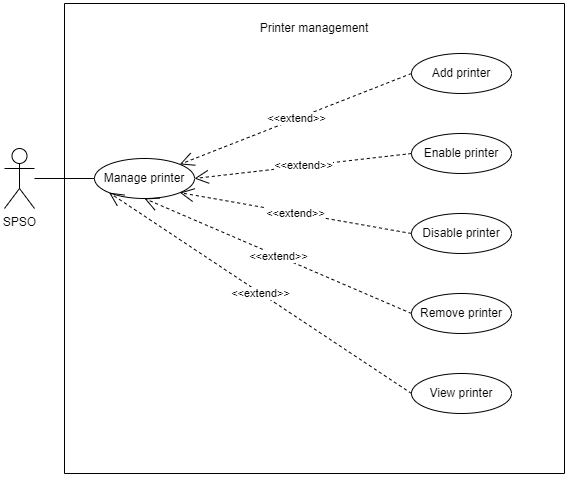
\includegraphics[width=1\textwidth]{Images/Requirement Elicitation/PM_Use-case.png}
        \caption{Use-case diagram cho chức năng quản lý máy in}
        \label{fig:arch}
    \end{center}
\end{figure}
\subsubsubsection{Use-case scenario}
\textbf{Manage printer}\par
\begin{tabular}{|c|c|c|c|}
\hline Use case name: & \multicolumn{3}{|l|}{ Manage printer} \\
\hline Created by: & Lê Đình Huy & Last updated by: & $\begin{array}{l}\text { Lê Đình Huy } \\\end{array}$ \\
\hline Date created: & $25 / 09 / 2023$ & Date last updated: & $29 / 09 / 2023$\\
\hline Actors: & \multicolumn{3}{|c|}{ SPSO } \\
\hline Description: & \multicolumn{3}{|c|}{$\begin{array}{l}\text { Cho phép SPSO quản lý các máy in cũng như là xem danh sách các máy in.}\end{array}$} \\
\hline Trigger: & \multicolumn{3}{|c|}{ Chọn nút "Quản lý máy in" tại thanh điều hướng. } \\
\hline Preconditions: & \multicolumn{3}{|c|}{$\begin{array}{l}\text { - SPSO có tài khoản trên website } \\
\text { - SPSO đã đăng nhập thành công vào hệ thống } \\
\text { - Thiết bị của SPSO có kết nối mạng và kết nối với hệ thống }\\
\text { - SPSO có quyền quản lý máy in }\end{array}$} \\
\hline Postconditions: & \multicolumn{3}{|c|}{$\begin{array}{l}\text { Giao diện quản lý máy in hiển thị đối với SPSO.} \end{array}$} \\
\hline Normal Flows: & \multicolumn{3}{|c|}{$\begin{array}{l}\text { 1. SPSO chọn "Printer management" trên thanh điều hướng. } \\
\text { 2. Hệ thống hiển thị giao diện quản lý máy in gồm danh sách các}\\
\text{máy in và các nút thêm, xóa, xem, enable và disable. } \end{array}$} \\
\hline  Alternative Flows: & \multicolumn{3}{|c|}{$\begin{array}{l} 
\text {Không có}\end{array}$} \\
\hline Exceptions: & \multicolumn{3}{|c|}{$\begin{array}{l}
\text {Không có}\end{array}$} \\
\hline Note and issues: & \multicolumn{3}{|c|}{ Không có } \\
\hline
\end{tabular}

\vspace{1cm}
\textbf{Enable printer}\par
\begin{tabular}{|c|c|c|c|}
\hline Use case name: & \multicolumn{3}{|l|}{ Enable printer} \\
\hline Created by: & Lê Đình Huy & Last updated by: & $\begin{array}{l}\text { Lê Đình Huy } \\\end{array}$ \\
\hline Date created: & $25 / 09 / 2023$ & Date last updated: & $29 / 09 / 2023$\\
\hline Actors: & \multicolumn{3}{|c|}{ SPSO } \\
\hline Description: & \multicolumn{3}{|c|}{$\begin{array}{l}\text { Cho phép SPSO kích hoạt một máy in. }\end{array}$} \\
\hline Trigger: & \multicolumn{3}{|c|}{ Chọn nút "Enable" cho một máy in tại giao diện quản lý máy in. } \\
\hline Preconditions: & \multicolumn{3}{|c|}{$\begin{array}{l}\text { - SPSO có tài khoản trên website } \\
\text { - SPSO đã đăng nhập thành công vào hệ thống } \\
\text { - Thiết bị của SPSO có kết nối mạng và kết nối với hệ thống }\\
\text { - SPSO có quyền quản lý máy in }\end{array}$} \\
\hline Postconditions: & \multicolumn{3}{|c|}{$\begin{array}{l}\text { Dữ liệu về máy in đã được update trong database và trên giao diện website.} \end{array}$} \\
\hline Normal Flows: & \multicolumn{3}{|c|}{$\begin{array}{l}\text { 1. SPSO chọn "Enable" cho một máy in.} \\
\text { 2. SPSO xác nhận thao tác. } \\
\text { 3. Hệ thống cập nhật dữ liệu trong database và website. }\end{array}$} \\
\hline  Alternative Flows: & \multicolumn{3}{|c|}{$\begin{array}{l} 
\text {Không có}\end{array}$} \\
\hline Exceptions: & \multicolumn{3}{|c|}{$\begin{array}{l}
\textbf { E1: Tại bước 2 } \\
\text { 2.1 SPSO không xác nhận thay đổi.} \\
\text { 2.2 Hệ thống xóa tất cả những thay đổi SPSO vừa thực hiện,} \\
\text { giao diện vẫn giữ nguyên ban đầu.} \\
\text { Use-case dừng lại.} 
\text {}\end{array}$} \\
\hline Note and issues: & \multicolumn{3}{|c|}{ Không có } \\
\hline
\end{tabular}

\vspace{1cm}
\textbf{Disable printer}\par
\begin{tabular}{|c|c|c|c|}
\hline Use case name: & \multicolumn{3}{|l|}{ Disable printer} \\
\hline Created by: & Lê Đình Huy & Last updated by: & $\begin{array}{l}\text { Lê Đình Huy } \\\end{array}$ \\
\hline Date created: & $25 / 09 / 2023$ & Date last updated: & $29 / 09 / 2023$\\
\hline Actors: & \multicolumn{3}{|c|}{ SPSO } \\
\hline Description: & \multicolumn{3}{|c|}{$\begin{array}{l}\text { Cho phép SPSO vô hiệu hóa một máy in. }\end{array}$} \\
\hline Trigger: & \multicolumn{3}{|c|}{ Chọn nút "Disable" cho một máy in tại giao diện quản lý máy in. } \\
\hline Preconditions: & \multicolumn{3}{|c|}{$\begin{array}{l}\text { - SPSO có tài khoản trên website } \\
\text { - SPSO đã đăng nhập thành công vào hệ thống } \\
\text { - Thiết bị của SPSO có kết nối mạng và kết nối với hệ thống }\\
\text { - SPSO có quyền quản lý máy in }\end{array}$} \\
\hline Postconditions: & \multicolumn{3}{|c|}{$\begin{array}{l}\text { Dữ liệu về máy in đã được update trong database và trên giao diện website.} \end{array}$} \\
\hline Normal Flows: & \multicolumn{3}{|c|}{$\begin{array}{l}\text { 1. SPSO chọn "Disable" cho một máy in.} \\
\text { 2. SPSO xác nhận thao tác. } \\
\text { 3. Hệ thống cập nhật dữ liệu trong database và website. }\end{array}$} \\
\hline  Alternative Flows: & \multicolumn{3}{|c|}{$\begin{array}{l} 
\text {Không có}\end{array}$} \\
\hline Exceptions: & \multicolumn{3}{|c|}{$\begin{array}{l}
\textbf { E1: Tại bước 2 } \\
\text { 2.1 SPSO không xác nhận thay đổi.} \\
\text { 2.2 Hệ thống xóa tất cả những thay đổi SPSO vừa thực hiện,} \\
\text { giao diện vẫn giữ nguyên ban đầu.} \\
\text { Use-case dừng lại.} 
\text {}\end{array}$} \\
\hline Note and issues: & \multicolumn{3}{|c|}{ Không có } \\
\hline
\end{tabular}

\vspace{1cm}
\textbf{Remove printer}\par
\begin{tabular}{|c|c|c|c|}
\hline Use case name: & \multicolumn{3}{|l|}{ Remove printer} \\
\hline Created by: & Lê Đình Huy & Last updated by: & $\begin{array}{l}\text { Lê Đình Huy } \\\end{array}$ \\
\hline Date created: & $25 / 09 / 2023$ & Date last updated: & $29 / 09 / 2023$\\
\hline Actors: & \multicolumn{3}{|c|}{ SPSO } \\
\hline Description: & \multicolumn{3}{|c|}{$\begin{array}{l}\text { Cho phép SPSO xóa một máy in. }\end{array}$} \\
\hline Trigger: & \multicolumn{3}{|c|}{ Chọn nút "Xóa" cho một máy in tại giao diện quản lý máy in. } \\
\hline Preconditions: & \multicolumn{3}{|c|}{$\begin{array}{l}\text { - SPSO có tài khoản trên website } \\
\text { - SPSO đã đăng nhập thành công vào hệ thống } \\
\text { - Thiết bị của SPSO có kết nối mạng và kết nối với hệ thống }\\
\text { - SPSO có quyền quản lý máy in }\end{array}$} \\
\hline Postconditions: & \multicolumn{3}{|c|}{$\begin{array}{l}\text { Dữ liệu về máy in đã được update trong database và trên giao diện website.} \end{array}$} \\
\hline Normal Flows: & \multicolumn{3}{|c|}{$\begin{array}{l}\text { 1. SPSO chọn "Xóa" cho một máy in.} \\
\text { 2. SPSO xác nhận thao tác. } \\
\text { 3. Hệ thống cập nhật dữ liệu trong database và website. }\end{array}$} \\
\hline  Alternative Flows: & \multicolumn{3}{|c|}{$\begin{array}{l} 
\text {Không có}\end{array}$} \\
\hline Exceptions: & \multicolumn{3}{|c|}{$\begin{array}{l}
\textbf { E1: Tại bước 2 } \\
\text { 2.1 SPSO không xác nhận thay đổi.} \\
\text { 2.2 Hệ thống xóa tất cả những thay đổi SPSO vừa thực hiện,} \\
\text { giao diện vẫn giữ nguyên ban đầu.} \\
\text { Use-case dừng lại.} 
\text {}\end{array}$} \\
\hline Note and issues: & \multicolumn{3}{|c|}{ Không có } \\
\hline
\end{tabular}

\vspace{1cm}
\textbf{Add printer}\par
\begin{tabular}{|c|c|c|c|}
\hline Use case name: & \multicolumn{3}{|l|}{ Add printer} \\
\hline Created by: & Lê Đình Huy & Last updated by: & $\begin{array}{l}\text { Lê Đình Huy } \\\end{array}$ \\
\hline Date created: & $25 / 09 / 2023$ & Date last updated: & $29 / 09 / 2023$\\
\hline Actors: & \multicolumn{3}{|c|}{ SPSO } \\
\hline Description: & \multicolumn{3}{|c|}{$\begin{array}{l}\text { Cho phép SPSO thêm một máy in. }\end{array}$} \\
\hline Trigger: & \multicolumn{3}{|c|}{ Chọn nút "Thêm máy in" tại giao diện quản lý máy in. } \\
\hline Preconditions: & \multicolumn{3}{|c|}{$\begin{array}{l}\text { - SPSO có tài khoản trên website } \\
\text { - SPSO đã đăng nhập thành công vào hệ thống } \\
\text { - Thiết bị của SPSO có kết nối mạng và kết nối với hệ thống }\\
\text { - SPSO có quyền quản lý máy in }\end{array}$} \\
\hline Postconditions: & \multicolumn{3}{|c|}{$\begin{array}{l}\text { Dữ liệu về máy in đã được update trong database và trên giao diện website.} \end{array}$} \\
\hline Normal Flows: & \multicolumn{3}{|c|}{$\begin{array}{l}\text { 1. SPSO chọn "Thêm máy in" tại giao diện quản lý máy in. } \\
\text {2. Hệ thống hiển thị biểu mẫu các thông tin của máy in mới. } \\
\text {3. SPSO điền biểu mẫu. } \\
\text {4. SPSO xác nhận thao tác. } \\
\text {5. Hệ thống cập nhật dữ liệu trong database và website. }\end{array}$} \\
\hline  Alternative Flows: & \multicolumn{3}{|c|}{$\begin{array}{l} 
\text {Không có}\end{array}$} \\
\hline Exceptions: & \multicolumn{3}{|c|}{$\begin{array}{l}
\textbf { E1: Tại bước 4 } \\
\text { 4.1 SPSO không xác nhận thay đổi.} \\
\text { 4.2 Hệ thống xóa tất cả những thay đổi SPSO vừa thực hiện,} \\
\text { giao diện vẫn giữ nguyên ban đầu.} \\
\text { Use-case dừng lại.} 
\text {}\end{array}$} \\
\hline Note and issues: & \multicolumn{3}{|c|}{ Không có } \\
\hline
\end{tabular}

\vspace{1cm}
\textbf{View printer}\par
\begin{tabular}{|c|c|c|c|}
\hline Use case name: & \multicolumn{3}{|l|}{ View printer} \\
\hline Created by: & Lê Đình Huy & Last updated by: & $\begin{array}{l}\text { Lê Đình Huy } \\\end{array}$ \\
\hline Date created: & $17 / 11 / 2023$ & Date last updated: & $17 / 11 / 2023$\\
\hline Actors: & \multicolumn{3}{|c|}{ SPSO } \\
\hline Description: & \multicolumn{3}{|c|}{$\begin{array}{l}\text { Cho phép SPSO xem thông tin của một máy in. }\end{array}$} \\
\hline Trigger: & \multicolumn{3}{|c|}{ Chọn nút "i" cho một máy in tại giao diện quản lý máy in. } \\
\hline Preconditions: & \multicolumn{3}{|c|}{$\begin{array}{l}\text { - SPSO có tài khoản trên website } \\
\text { - SPSO đã đăng nhập thành công vào hệ thống } \\
\text { - Thiết bị của SPSO có kết nối mạng và kết nối với hệ thống }\\
\text { - SPSO có quyền quản lý máy in }\end{array}$} \\
\hline Postconditions: & \multicolumn{3}{|c|}{$\begin{array}{l}\text { Thông tin máy in được hiển thị trên giao diện của người dùng.} \end{array}$} \\
\hline Normal Flows: & \multicolumn{3}{|c|}{$\begin{array}{l}\text { 1. Chọn nút "i" cho một máy in tại giao diện quản lý máy in. }  \\
\text {2. Hệ thống hiển thị các thông tin của máy in. } \end{array}$} \\
\hline  Alternative Flows: & \multicolumn{3}{|c|}{$\begin{array}{l} 
\text {Không có}\end{array}$} \\
\hline Exceptions: & \multicolumn{3}{|c|}{$\begin{array}{l}
\text {Không có}\end{array}$} \\
\hline Note and issues: & \multicolumn{3}{|c|}{ Không có } \\
\hline
\end{tabular}

\subsubsection{Sửa danh mục định dạng tệp cho phép in}
\subsubsubsection{Use-case diagram}
\begin{figure}[H]
    \begin{center}
        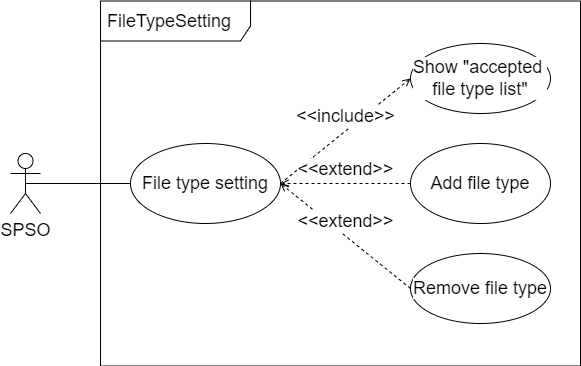
\includegraphics[width=1\textwidth]{Images/Requirement Elicitation/FileTypeSetting_Use-case.png}
        \caption{Use-case diagram cho những tính năng liên quan đến in ấn}
        \label{fig:arch}
    \end{center}
\end{figure}
\subsubsubsection{Use-case scenario}
\begin{tabular}{|c|c|c|c|}
\hline Use case name: & \multicolumn{3}{|l|}{ File type setting} \\
\hline Created by: & Phan Lê Nhật Minh & Last updated by: & $\begin{array}{l}\text { Phan Lê Nhật Minh } \\\end{array}$ \\
\hline Date created: & $28 / 09 / 2023$ & Date last updated: & $28 / 09 / 2023$\\
\hline Actors: & \multicolumn{3}{|c|}{ SPSO } \\
\hline Description: & \multicolumn{3}{|c|}{$\begin{array}{l}
\text { SPSO dùng tính năng chỉnh sửa những định dạng tệp được phép sử dụng } \\
\end{array}$} \\

\hline Trigger: & \multicolumn{3}{|l|}
{$\begin{array}{l}
\text{SPSO: Chọn nút "File Type Setting" tại thanh điều hướng. } \\
\end{array}$} \\

\hline Preconditions: & \multicolumn{3}{|l|}{$\begin{array}{l}\text { - SPSO có tài khoản trên website } \\
\text { - SPSO đã đăng nhập thành công vào hệ thống với quyền hạn SPSO}\\
\text { - Thiết bị của SPSO có kết nối mạng và kết nối với hệ thống }\end{array}$} \\

\hline Postconditions: & \multicolumn{3}{|l|}{$\begin{array}{l}\text { Dữ liệu về định dạng tệp in  (file type) cho phép đã được update trong database.} \end{array}$} \\
\hline Normal Flows: & \multicolumn{3}{|l|}
{$\begin{array}{l}\text { 1. SPSO chọn "File Type Setting" trên thanh điều hướng,}\\
\text{ hệ thống hiển thị những định dạng file hiện tại } \\
\text { 2. SPSO chọn "Add file type",  Hệ thống hiển thị ô điền } \\
\text { 3. SPSO nhập file type mới gồm 3 chữ cái trở lên}\\
\text { 4. SPSO chọn Apply.} \\
\text{Hệ thống xác nhận thay đổi, cập nhật lại database,}\\
\text{ quay lại giao diện trang chủ }
\end{array}$} \\
\hline  Alternative Flows: & \multicolumn{3}{|l|}
{$
\begin{array}{l}\textbf { A1: Tại bước 2 } \\
\text { 2.1 SPSO chọn "Remove file type", Hệ thống hiển thị ô điền } \\
\text {Tiếp tục tại bước 3 trong Normal Flows.} \\
\end{array}
$} \\

\hline Exceptions: & \multicolumn{3}{|l|}
{$
\begin{array}{l}
\textbf { E1: Tại bước 4 } \\
\text { 4.1 SPSO chọn Apply, Hệ thống phát hiện thay đổi không hợp lệ.} \\
\text { 4.2 Hệ thống xóa tất cả những thay đổi vừa thực hiện,} \\
\text { giao diện vẫn giữ nguyên ban đầu.  Quay lại bước 2.} 
\text {}\end{array}
$} \\
\hline Note and issues: & \multicolumn{3}{|c|}{ Không có } \\
\hline
\end{tabular}

\subsubsection{Chọn ngày tặng giấy}
\subsubsubsection{Use-case diagram}
\begin{figure}[H]
    \begin{center}
        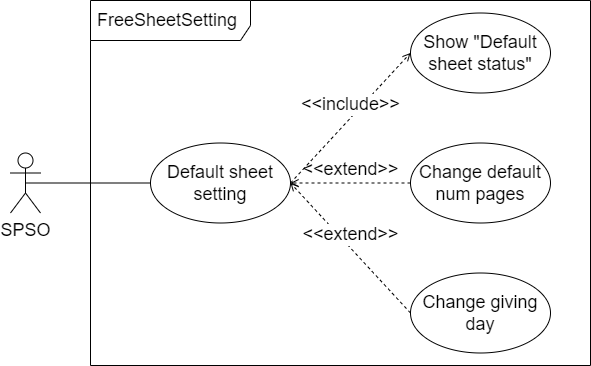
\includegraphics[width=1\textwidth]{Images/Requirement Elicitation/FreeSheetSetting_Use-case.png}
        \caption{Use-case diagram cho tính năng quà tặng}
        \label{fig:arch}
    \end{center}
\end{figure}
\subsubsubsection{Use-case scenario}
\begin{tabular}{|c|c|c|c|}
\hline Use case name: & \multicolumn{3}{|l|}{ Free sheet gifting} \\
\hline Created by: & Phan Lê Nhật Minh & Last updated by: & $\begin{array}{l}\text { Phan Lê Nhật Minh } \\\end{array}$ \\
\hline Date created: & $28 / 09 / 2023$ & Date last updated: & $28 / 09 / 2023$\\
\hline Actors: & \multicolumn{3}{|c|}{ SPSO } \\
\hline Description: & \multicolumn{3}{|c|}{$\begin{array}{l}
\text { SPSO dùng tính năng tặng quà cho user } \\
\end{array}$} \\

\hline Trigger: & \multicolumn{3}{|l|}
{$\begin{array}{l}
\text{SPSO: Chọn nút "Free sheet setting" tại thanh điều hướng. } \\
\end{array}$} \\

\hline Preconditions: & \multicolumn{3}{|l|}{$\begin{array}{l}\text { - SPSO có tài khoản trên website } \\
\text { - SPSO đã đăng nhập thành công vào hệ thống với quyền hạn SPSO}\\
\text { - Thiết bị của SPSO có kết nối mạng và kết nối với hệ thống }\end{array}$} \\

\hline Postconditions: & \multicolumn{3}{|l|}{$\begin{array}{l}\text { Dữ liệu về ngày tặng quà, số giấy đã được update trong database} \\
\text { và trên giao diện website.}
\end{array}$} \\
\hline Normal Flows: & \multicolumn{3}{|l|}
{$\begin{array}{l}\text { 1. SPSO chọn "Free sheet setting" trên thanh điều hướng,}\\
\text{ hệ thống hiển thị trang "Free sheet status" trước đó } \\
\text { 2. SPSO chọn "Change default num pages",  Hệ thống hiển thị ô điền } \\
\text { 3. SPSO nhập dữ liệu }\\
\text { 4. SPSO chọn Apply}
\text{ Hệ thống xác nhận thay đổi, cập nhật lại database, }\\
\text{ quay lại giao diện trang chủ }
\end{array}$} \\
\hline  Alternative Flows: & \multicolumn{3}{|l|}
{$
\begin{array}{l}\textbf { A1: Tại bước 2 } \\
\text { 2.1 SPSO chọn "Change giving day", Hệ thống hiển thị ô điền } \\
\text {Tiếp tục tại bước 3 trong Normal Flows.} \\
\end{array}
$} \\

\hline Exceptions: & \multicolumn{3}{|l|}
{$
\begin{array}{l}
\textbf { E1: Tại bước 4 } \\
\text { 4.1 SPSO chọn Apply, Hệ thống phát hiện thay đổi không hợp lệ.} \\
\text { 4.2 Hệ thống xóa tất cả những thay đổi vừa thực hiện,} \\
\text { giao diện vẫn giữ nguyên ban đầu.  Quay lại bước 2.} 
\text {}\end{array}
$} \\
\hline Note and issues: & \multicolumn{3}{|c|}{ Không có } \\
\hline
\end{tabular}

\subsubsection{Phản hồi}
\subsubsubsection{Use-case diagram}
\begin{figure}[H]
    \begin{center}
        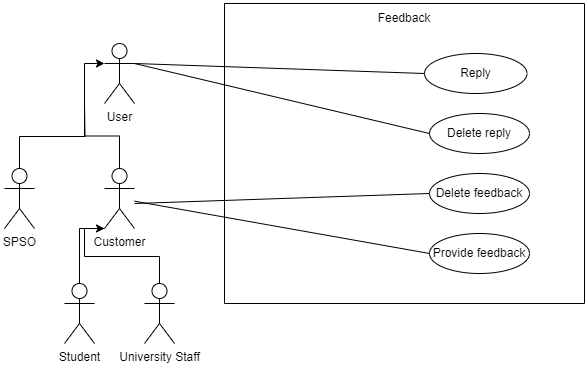
\includegraphics[width=1\textwidth]{Images/Requirement Elicitation/Feedback_Use-case.png}
        \caption{Use-case diagram cho chức năng phản hồi và khiếu nại}
        \label{fig:arch}
    \end{center}
\end{figure}

\subsubsubsection{Use-case scenario}
\pagebreak
\textbf{Use-case Provide feedback}\par
\vspace{0.5cm}
\begin{tabular}{|c|c|c|c|}
\hline Use case name: & \multicolumn{3}{|l|}{ Provide feedback} \\
\hline Created by: & Lê Đình Huy & Last updated by: & $\begin{array}{l}\text { Lê Đình Huy } \\\end{array}$ \\
\hline Date created: & $25 / 09 / 2023$ & Date last updated: & $29 / 09 / 2023$\\
\hline Actors: & \multicolumn{3}{|c|}{ Khách hàng } \\
\hline Description: & \multicolumn{3}{|c|}{$\begin{array}{l}\text { Cho phép khách hàng cung cấp các phản hồi về hệ thống. } \end{array}$} \\
\hline Trigger: & \multicolumn{3}{|c|}{ Chọn nút "Add feedback" trong giao diện feedback. } \\
\hline Preconditions: & \multicolumn{3}{|c|}{$\begin{array}{l}\text { - Khách hàng có tài khoản trên website } \\
\text { - Khách hàng đã đăng nhập thành công vào hệ thống } \\
\text { - Thiết bị của khách hàng có kết nối mạng và kết nối với hệ thống }\\
\text { - Khách hàng có quyền cung cấp feedback }\end{array}$} \\
\hline Postconditions: & \multicolumn{3}{|c|}{$\begin{array}{l}\text { Feedback được gửi lên hệ thống và hiển thị trong mục "Feedback".}\\
\text{ của khách hàng.} \end{array}$} \\
\hline Normal Flows: & \multicolumn{3}{|c|}{$\begin{array}{l}\text { 1. Khách hàng chọn "Feedback" tại thanh điều hướng.} \\
\text { 2. Hệ thống hiển thị giao diện Feedback.} \\
\text { 3. Khách hàng chọn "Add feedback".} \\
\text { 4. Hệ thống hiển thị biểu mẫu các thông tin của một feedback.} \\
\text { 5. Khách hàng điền biểu mẫu.  }\\
\text { 6. Khách hàng xác nhận thao tác.  }\\
\text { 7. Feedback được gửi lên hệ thống và hiển thị trong giao}\\
\text{diện Feedback của chính khách hàng đó và SPSO.  }
\end{array}$} \\
\hline  Alternative Flows: & \multicolumn{3}{|c|}{$\begin{array}{l}\text {Không có } \end{array}$} \\
\hline Exceptions: & \multicolumn{3}{|c|}{$\begin{array}{l}
\textbf { E1: Tại bước 6 } \\
\text { 6.1 Khách hàng không xác nhận.} \\
\text { 6.2 Hệ thống xóa tất cả những thay đổi khách hàng vừa thực } \\
\text { hiện, giao diện vẫn giữ nguyên ban đầu.} \\
\text { Use-case dừng lại.} 
\text {}\end{array}$} \\
\hline Note and issues: & \multicolumn{3}{|c|}{ Không có } \\
\hline
\end{tabular}

\pagebreak
\textbf{Use-case Delete feedback}\par
\vspace{0.5cm}
\begin{tabular}{|c|c|c|c|}
\hline Use case name: & \multicolumn{3}{|l|}{ Delete feedback} \\
\hline Created by: & Lê Đình Huy & Last updated by: & $\begin{array}{l}\text { Lê Đình Huy } \\\end{array}$ \\
\hline Date created: & $25 / 09 / 2023$ & Date last updated: & $15 / 10 / 2023$\\
\hline Actors: & \multicolumn{3}{|c|}{ Khách hàng } \\
\hline Description: & \multicolumn{3}{|c|}{$\begin{array}{l}\text { Cho phép khách hàng xóa các phản hồi của mình về hệ thống. } \end{array}$} \\
\hline Trigger: & \multicolumn{3}{|c|}{ Chọn nút "Delete" cho feedback cần xóa. } \\
\hline Preconditions: & \multicolumn{3}{|c|}{$\begin{array}{l}\text { - Khách hàng có tài khoản trên website } \\
\text { - Khách hàng đã đăng nhập thành công vào hệ thống } \\
\text { - Thiết bị của khách hàng có kết nối mạng và kết nối với hệ thống }\\
\text { - Khách hàng có quyền xóa feedback đó }\end{array}$} \\
\hline Postconditions: & \multicolumn{3}{|c|}{$\begin{array}{l}\text { Feedback được chọn và tất cả Reply trong nó bị xóa khỏi hệ thống. } \end{array}$} \\
\hline Normal Flows: & \multicolumn{3}{|c|}{$\begin{array}{l}\text { 1. Khách hàng chọn "Feedback" tại thanh điều hướng.} \\
\text { 2. Hệ thống hiển thị giao diện Feedback gồm danh sách các feedback.} \\
\text{  3. Khách hàng chọn "Delete" cho một feedback.}\\
\text { 4. Khách hàng xác nhận thao tác.  }\\
\text { 5. Feedback và các reply trong nó được xóa khỏi hệ thống.}\end{array}$} \\
\hline  Alternative Flows: & \multicolumn{3}{|c|}{$\begin{array}{l}
\textbf{A1: Tại bước 3}\\
\text { 3.1 Khách hàng chọn "View" một feedback.} \\
\text { 3.2 Hệ thống hiển thị nội dung của feedback.} \\
\text { 3.3 Khách hàng chọn "Delete".  }\\
\text {Tiếp tục tại bước 4 trong Normal Flows.} 
\end{array}$} \\
\hline Exceptions: & \multicolumn{3}{|c|}{$\begin{array}{l}
\textbf { E1: Tại bước 4 } \\
\text { 4.1 Khách hàng không xác nhận.} \\
\text { 4.2 Hệ thống xóa tất cả những thay đổi khách hàng vừa thực } \\
\text { hiện, giao diện vẫn giữ nguyên ban đầu.} \\
\text { Use-case dừng lại.} 
\text {}\end{array}$} \\
\hline Note and issues: & \multicolumn{3}{|c|}{ Không có } \\
\hline
\end{tabular}

\pagebreak
\textbf{Use-case Reply}\par
\vspace{0.5cm}
\begin{tabular}{|c|c|c|c|}
\hline Use case name: & \multicolumn{3}{|l|}{ Reply} \\
\hline Created by: & Lê Đình Huy & Last updated by: & $\begin{array}{l}\text { Lê Đình Huy } \\\end{array}$ \\
\hline Date created: & $25 / 09 / 2023$ & Date last updated: & $29 / 09 / 2023$\\
\hline Actors: & \multicolumn{3}{|c|}{ User (Customer và SPSO) } \\
\hline Description: & \multicolumn{3}{|c|}{$\begin{array}{l}\text { Cho phép User trả lời các Feedback của Customer.}\end{array}$} \\
\hline Trigger: & \multicolumn{3}{|c|}{ Chọn nút "Reply" trong giao diện xem của feedback đó. } \\
\hline Preconditions: & \multicolumn{3}{|c|}{$\begin{array}{l}\text { - User có tài khoản trên website } \\
\text { - User đã đăng nhập thành công vào hệ thống } \\
\text { - Thiết bị của User có kết nối mạng và kết nối với hệ thống }\\
\text { - User có quyền reply }\end{array}$} \\
\hline Postconditions: & \multicolumn{3}{|c|}{$\begin{array}{l}\text { Reply được gửi lên hệ thống và hiển thị trên website. } \end{array}$} \\
\hline Normal Flows: & \multicolumn{3}{|c|}{$\begin{array}{l}\text { 1. User chọn "Feedback" tại thanh điều hướng.} \\
\text { 2. Hệ thống hiển thị giao diện Feedback gồm danh sách các feedback.} \\
\text { 3. User chọn "View" một feedback.} \\
\text { 4. Hệ thống hiển thị giao diện của một feedback.} \\
\text { 5. User chọn "Reply".  }\\
\text { 6. Hệ thống hiển thị biểu mẫu của Reply. }\\
\text { 7. User điền biểu mẫu.  }\\
\text { 8. User xác nhận thao tác.  }\\
\text { 9. Reply được gửi lên hệ thống và hiển thị trên website.}\end{array}$} \\
\hline  Alternative Flows: & \multicolumn{3}{|c|}{$\begin{array}{l}
\text {Không có}\end{array}$} \\
\hline Exceptions: & \multicolumn{3}{|c|}{$\begin{array}{l}
\textbf { E1: Tại bước 8 } \\
\text { 8.1 User không xác nhận.} \\
\text { 8.2 Hệ thống xóa tất cả những thay đổi User vừa thực } \\
\text { hiện, giao diện vẫn giữ nguyên ban đầu.} \\
\text { Use-case dừng lại.} 
\text {}\end{array}$} \\
\hline Note and issues: & \multicolumn{3}{|c|}{ Không có } \\
\hline
\end{tabular}

\pagebreak
\textbf{Use-case Delete reply}\par
\vspace{0.5cm}
\begin{tabular}{|c|c|c|c|}
\hline Use case name: & \multicolumn{3}{|l|}{ Delete reply} \\
\hline Created by: & Lê Đình Huy & Last updated by: & $\begin{array}{l}\text { Lê Đình Huy } \\\end{array}$ \\
\hline Date created: & $25 / 09 / 2023$ & Date last updated: & $29 / 09 / 2023$\\
\hline Actors: & \multicolumn{3}{|c|}{ User (Customer và SPSO) } \\
\hline Description: & \multicolumn{3}{|c|}{$\begin{array}{l}\text { Cho phép User xóa Reply của mình.} \end{array}$} \\
\hline Trigger: & \multicolumn{3}{|c|}
{$\begin{array}{l}
\text { Chọn nút "Delete" cho một reply của mình trong giao diện xem} \\
\text {của feedback đó. } \end{array}$} \\
\hline Preconditions: & \multicolumn{3}{|c|}{$\begin{array}{l}\text { - User có tài khoản trên website } \\
\text { - User đã đăng nhập thành công vào hệ thống } \\
\text { - Thiết bị của User có kết nối mạng và kết nối với hệ thống }\\
\text { - User có quyền xóa reply đó}\end{array}$} \\
\hline Postconditions: & \multicolumn{3}{|c|}{$\begin{array}{l}\text { Reply được xóa khỏi hệ thống.} \end{array}$} \\
\hline Normal Flows: & \multicolumn{3}{|c|}{$\begin{array}{l}\text { 1. User chọn "Feedback" tại thanh điều hướng.} \\
\text { 2. Hệ thống hiển thị giao diện Feedback gồm danh sách các feedback.} \\
\text { 3. User chọn "View" một feedback.} \\
\text { 4. Hệ thống hiển thị giao diện của một feedback.} \\
\text { 5. User chọn "Delete" cho Reply cần xóa của mình.  }\\
\text { 6. User xác nhận thao tác.  }\\
\text { 7. Reply được xóa khỏi hệ thống.}\end{array}$} \\
\hline  Alternative Flows: & \multicolumn{3}{|c|}{$\begin{array}{l}\text {Không có}\end{array}$} \\
\hline Exceptions: & \multicolumn{3}{|c|}{$\begin{array}{l}
\textbf { E1: Tại bước 6 } \\
\text { 6.1 User không xác nhận.} \\
\text { 6.2 Hệ thống xóa tất cả những thay đổi User vừa thực } \\
\text { hiện, giao diện vẫn giữ nguyên ban đầu.} \\
\text { Use-case dừng lại.} 
\text {}\end{array}$} \\
\hline Note and issues: & \multicolumn{3}{|c|}{ Không có } \\
\hline
\end{tabular}

\pagebreak

\subsubsection{Lịch sử in}
\subsubsubsection{Use case diagram}
\begin{figure}[H]
    \begin{center}
        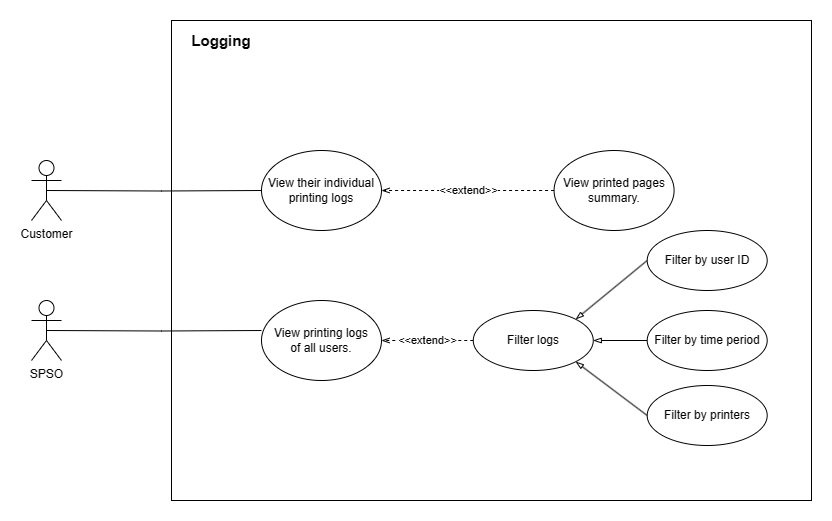
\includegraphics[width=1\textwidth]{Images/Requirement Elicitation/Logging_Use-case.png}
        \caption{Use-case diagram cho chức năng truy cập lịch sử in}
    \end{center}
\end{figure}

\subsubsubsection{Use-case scenario}
\pagebreak
\textbf{Use-case View printing logs of all users}\par
\vspace{0.5cm}
\begin{tabular}{|l|l|l|l|}
\hline Use case name: & \multicolumn{3}{|l|}{View printing logs of all users} \\
\hline Created by: & Phạm Đức Thắng & Last updated by: &  Phạm Đức Thắng \\
\hline Date created: & 28/09/2023 & Date last updated: & 28/09/2023\\
\hline Actors: & \multicolumn{3}{|l|}{ Student Printing Service Officer (SPSO) } \\
\hline Description: & \multicolumn{3}{|l|}{$\begin{array}{l}\text{Use case này cho phép SPSO truy cập toàn bộ lịch sử in ấn của tất cả } \\ \text{người dùng} \end{array}$} \\

\hline Trigger: & \multicolumn{3}{|l|}{SPSO click vào ô “View Printing History” trên thanh điều hướng.} \\
\hline Preconditions: & \multicolumn{3}{|l|}{$\begin{array}{l}\text {SPSO phải đăng nhập vào hệ thống. } \\
\text {Hệ thống được kết nối với cơ sở dữ liệu lưu trữ lịch sử người dùng.}\end{array}$} \\
\hline Postconditions: & \multicolumn{3}{|l|}{$\begin{array}{l}\text {SPSO đã truy cập thành công lịch sử in ấn của tất cả người dùng.} \\
\text {Dữ liệu lịch sử in ấn không bị thay đổi.}\end{array}$} \\
\hline Normal Flows: & \multicolumn{3}{|l|}{$\begin{array}{l}\text {1. SPSO click vào ô “View Printing History” trên thanh điều hướng. } \\
\text {2. Hệ thống hiển thị mặc định thông tin lịch sử in của tất cả người} \\
\text {dùng đã đăng ký cùng các bộ lọc (theo thời gian hoặc ID máy in) } \\
\text {và thanh tìm kiếm ID người dùng. } \\
\text {Thông tin hiển thị bao gồm: ID người sử dụng, ID máy in, tên file,  } \\
\text {thời điểm bắt đầu và kết thúc in, số trang in với mỗi kích thước trang. } \\
\text {Các thông tin được phân trang với tối đa 10 thông tin mỗi trang.}\end{array}$} \\
\hline  Alternative Flows: & \multicolumn{3}{|l|}{$\begin{array}{l}\textbf{A1: tại bước 2 } \\
\text {2a: SPSO sử dụng bộ lọc hoặc thanh tìm kiếm. } \\
\text {2b: Hệ thống chỉ hiển thị thông tin lịch sử in trong khoảng thời gian,} \\ 
\text {của máy in được chọn và/hoặc của người dùng có ID trên thanh tìm kiếm. }
\end{array}$} \\
\hline Exceptions: & \multicolumn{3}{|l|}{$\begin{array}{l}\textbf{E1: tại bước 2 } \\
\text {2a: SPSO sử dụng bộ lọc thời gian không hợp lệ (ngày bắt đầu sau ngày } \\
\text {kết thúc, ngày kết thúc sau ngày hiện tại).} \\
\text {2b: Hệ thống báo lỗi tương ứng và yêu cầu user nhập lại thông tin hợp lệ. } \\
\textbf{E2: tại bước 2 } \\
\text {2a: Nếu chưa có dữ liệu in hoặc không có dữ liệu in nào thỏa mãn điều } \\
\text {kiện bộ lọc, hệ thống hiển thị thông báo không có dữ liệu in. }\end{array}$} \\
\hline Note and issues: & \multicolumn{3}{|l|}{ } \\
\hline
\end{tabular}


\pagebreak
\textbf{Use-case View individual printing logs}\par
\vspace{0.5cm}
\begin{tabular}{|l|l|l|l|}
\hline Use case name: & \multicolumn{3}{|l|}{View individual printing logs} \\
\hline Created by: & Phạm Đức Thắng & Last updated by: & Phạm Đức Thắng \\
\hline Date created: & 28/09/2023 & Date last updated: & 28/09/2023 \\
\hline Actors: & \multicolumn{3}{|l|}{User} \\
\hline Description: & \multicolumn{3}{|l|}{Use case này cho phép người dùng truy cập lịch sử in ấn cá nhân.} \\
\hline Trigger: & \multicolumn{3}{|l|}{User click vào ô “View Printing History” trên thanh điều hướng.} \\
\hline Preconditions: & \multicolumn{3}{|l|}{$\begin{array}{l}
\text{User phải đăng nhập thành công vào hệ thống.} \\
\text{Hệ thống được kết nối với cơ sở dữ liệu lưu trữ lịch sử người dùng.}
\end{array}$} \\
\hline Postconditions: & \multicolumn{3}{|l|}{$\begin{array}{l}
\text{User truy cập thành công lịch sử in ấn cá nhân.} \\
\text{Dữ liệu lịch sử in ấn không bị thay đổi.}
\end{array}$} \\
\hline Normal Flows: & \multicolumn{3}{|l|}{$\begin{array}{l}
\text{1. User click vào ô “View Printing History” trên thanh điều hướng.} \\
\text{2. Hệ thống hiển thị trang lịch sử in cá nhân bao gồm thông tin lịch } \\
\text{sử in ấn cá nhân và các bộ lọc (theo khoảng thời gian và ID máy in). } \\
\text{Mỗi thông tin lịch sử in được hiển thị bao gồm: ID người dùng, ID máy} \\
\text{in, tên file, thời điểm bắt đầu và kết thúc in, số trang in ứng với mỗi} \\
\text{kích thước trang. Các thông tin được phân trang với tối đa 10 thông } \\
\text{tin mỗi trang.} \\
\end{array}$} \\
\hline Alternative Flows: & \multicolumn{3}{|l|}{$\begin{array}{l}
\textbf{A1: tại bước 2} \\
\text{2a: User sử dụng bộ lọc theo thời gian hoặc theo ID máy in.} \\
\text{2b: Hệ thống hiển thị thông tin lịch sử in thỏa mãn các điều kiện của } \\
\text{bộ lọc.}
\end{array}$} \\
\hline Exceptions: & \multicolumn{3}{|l|}{$\begin{array}{l}
\textbf{E1: tại bước 2} \\
\text{2a: User sử dụng bộ lọc thời gian không hợp lệ (ngày bắt đầu sau ngày
} \\
\text{kết thúc, ngày kết thúc sau ngày hiện tại).} \\
\text{2b: Hệ thống báo lỗi tương ứng và yêu cầu user nhập lại thông tin hợp lệ.} \\
\textbf{E2: tại bước 2} \\
\text{2a: Nếu chưa có dữ liệu lịch sử in hoặc không có dữ liệu lịch sử in nào} \\
\text{thỏa mãn điều kiện bộ lọc, hệ thống hiển thị thông báo không có dữ liệu } \\
\text{lịch sử in.} \\
\end{array}$} \\
\hline Notes and Issues: & \multicolumn{3}{|l|}{} \\
\hline
\end{tabular}





